\section{Pesquisa em engenharia de software}

%https://plato.stanford.edu/entries/computer-science/#Aca
%Scientific Output and Recognition: A Study in the Operation of the Reward System in Science

estudo de campo, field study, exploratory case study,

ou

Sample Surveys?

As pesquisas realizadas em engenharia de software possuem um leque estreito em
relação à abordagem e método de pesquisa utilizados  \cite{glass2002research}

Mais recentemente uma gama de novas abordagens tem sido introduzida, incluindo
abordagens qualitativas como grounded theory studies, ethnographies, and delphi
studies \cite{hazzan2010qualitative}.

Existe ainda muito desentendimento e confusão sobre a termilogia em pesquisas
da engenharia de software, por exemplo, quando se fala em métodos de pesquisa,
é comum listar estudos de caso, experimentos controlados, entrevistas, grounded
theory studies, e observational studies \cite{hazzan2010qualitative}.

Entretanto, esses métodos e técnisas são, de fato uma combinação de coisas
\cite{mcgrath1981dilemmatics}, e assim, não estão no mesmo nível de abstração.
Alguns pesquisadores referem-se a ``estudo de caso'' como uma ``estratégia'' ou
``abordagem'', outros falam disso como método de pesquisa.

Caracterizar um estudo como um ``estudo de caso'' ou um ``experimento'' não
agrega tanto valor em termos de distinção da pesquisa. Os
estudos de caso, por exemplo, podem ser descritivos, exploratórios ou
avaliativos, e mesmo dentro de cada um desses, o nível de ``controle'' que um
pesquisador (acredita que ele ou ela) exerce também varia.

Ao invés de discutir
métodos de pesquisa, acreditamos que é melhor pensar em uma ``estratégia de
pesquisa'', que representa um projeto de alto nível do estudo, semelhante ao
conceito de arquitetura (de um edifício ou sistema de software).

Semelhante à
forma como uma arquitetura de software tem um impacto significativo nos
atributos de qualidade de um sistema, como desempenho e confiabilidade, uma
``estratégia de pesquisa'', também, tem um impacto significativo sobre o que pode e
não pode ser alcançado em um estudo em termos de aquisição de novos
conhecimentos e uma compreensão mais profunda dos fenômenos.

Esta consciência ainda não é amplamente reconhecida na comunidade de pesquisa
SE \cite{stol2015holistic}.

\section{O papel do software na reprodutibilidade}

% Falar de:
% * reprodutibilidade como prática do método científico experimental
% * definição de reprodutibilidade, variações, aplicações, formatos, ...
% * software como artefato (similar a dados) e software como aparato (similar a telescopio)
% * impactoda falta de sustentabilidade na reprodutibilidade em engenharia de software experimental
% * ...

%
%8.1. The importance of replication for empirical studies of software evolution
%Public availability of the data used for empirical studies is crucial. A theory of software
%evolution must be based on empirical results, verifiable and repeatable, and made on
%a large scale, so that conclusions with statistical significance can be achieved [Sjøberg
%et al. 2008]. If software evolution is analyzed with data that is not available to third
%parties, it cannot be verified, repeated and replicated. It is dangerous to build a theory
%on top of empirical studies that do not fulfill those requirements.
%Empirical studies of software evolution should conform to the guidelines suggested
%for empirical software engineering [Kitchenham et al. 2002; Kitchenham et al. 2008].
%The entry barrier for repeatable empirical studies can be lowered using reusable
%datasets such as FLOSSMetrics [Herraiz et al. 2009], FLOSSMole [Howison et al.
%2006], the Qualitas Corpus [Tempero et al. 2010] or the UCI Sourcerer Dataset [Lopes
%et al. 2010]. These datasets aim to achieve replicability of empirical studies of software
%development and evolution. Replicability is a concern recently raised in the empirical
%software engineering research community [González-Barahona and Robles 2012], with
%many authors highlighting its potential benefits [Robles and German 2010; Shull et al.
%2008; Brooks et al. 2008; Barr et al. 2010].
%However, Kitchenham warns about some of the problems that may arise with repli-
%cation and sharing [Kitchenham 2008],in particular when reusing the so-called labo-
%ratory packages. If these packages are only gathered once and reused many times, that
%would amplify the probable errors that occur during the gathering phase. The avail-
%ability of datasets does not remove the need for new datasets, that can be used to test
%the correctness of previous results. In any case, this does not invalidate the previous
%argument: software evolution studies must be replicable, either by reusing third party
%datasets and tools, or by making their data and/or tools publicly available.
%\cite{The evolution of the laws of software evolution. A discussion based on a systematic literature review}
%
%
%
%Abstract. Experimentation has played a major role in scientific
%advancement. Replication is one of the essentials of the experimental
%methods. In replications, experiments are repeated aiming to check their
%results. Successful replication increases the validity and reliability of the
%outcomes observed in an experiment.
%There is debate about the best way of running replications of Soft-
%ware Engineering (SE) experiments. Some of the questions that have
%cropped up in this debate are, “Should replicators reuse the baseline ex-
%periment materials? Which is the adequate sort of communication among
%experimenters and replicators if any? What elements of the experimental
%structure can be changed and still be considered a replication instead of
%a new experiment?”. A deeper understanding of the concept of replica-
%tion should help to clarify these issues as well as increase and improve
%replications in SE experimental practices.
%In this chapter, we study the concept of replication in order to gain
%insight. The chapter starts with an introduction to the importance of
%replication and the state of replication in ESE. Then we discuss replica-
%tion from both the statistical and scientific viewpoint. Based on a review
%of the diverse types of replication used in other scientific disciplines, we
%identify the different types of replication that are feasible to be run in
%our discipline. Finally, we present the different purposes that replication
%can serve in Experimental Software Engineering (ESE).
%\cite{Replication of Software Engineering Experiments}
%
%Experiment replication is a key feature of
%experimentation in any scientific or technological field.
%Intuitively, replication means the repetition of an
%experiment to double-check its results [18]. The replication
%of an experiment produces new results, which, through
%comparison with the outcomes of the original experiment
%(or other replications), increase or decrease the credibility
%of the results. After several replications have increased the
%credibility of the results, the small fragment of knowledge
%that the experiment was trying to ascertain is more mature.
%This way, replication helps to produce an experimentally
%backed body of knowledge. The software engineering (SE)
%community has been trying for years to replicate
%experiments to generate fragments of knowledge.
%Almost all the replication attempts to date have turned
%out to be unsatisfactory (the credibility of the results has
%not increased), mainly due to variations in the experimental
%conditions from one replication to another [5], [12], [13],
%[17]. Only when the same researchers have carried out the
%replication at the same site has a replication been
%successfully achieved ([10], [14], [19]).
%Unwanted variations in the experimental conditions are a
%consequence of it being extremely difficult to describe a SE
%experiment in enough detail for another researcher to
%control the replication setting and replicate it exactly [20].
%When the context of an experiment is suitably controlled
%(which is much easier for the same researchers working in
%the same settings), replications have been satisfactory. It is
%very hard to properly control the replication context in
%experimentally immature fields dealing with human beings
%working in complex settings, like SE. The context of a SE
%experiment covers hundreds of variables, and we do not
%know yet which are of major importance.
%Because the context is so complex, a lot of information
%is needed about the experiment if it is to be satisfactorily
%replicated. For example, when replicating experiments
%about SE design techniques, not only do researchers need
%to know which techniques were examined, but also how the
%techniques were applied, how the subjects were trained,
%what knowledge these subjects already had, etc.
%To help experimenters to repeat a SE experiment as
%exactly as possible, replication packages have been
%developed. They transmit the necessary information about
%an experiment for other experimenters. The information
%that a replication package should contain has evolved over
%the years, as shown in [3], [9], [15], [16]. Even with these
%replication packages, though, several studies have brought
%attention to the fact that there are still very few SE
%replications [5]. For some reason, experimental packages
%are not as helpful as they were expected to be. Also, there
%are authors against the use of replication packages [8]. This
%suggests that we might be dealing with the issue of SE
%experiment replication from too naïve a perspective.
%\cite{Using Differences among Replications of Software Engineering Experiments to Gain Knowledge}

%https://pt.wikipedia.org/wiki/Empirismo
%
%O empirismo causou uma grande revolução na ciência, pois graças à valorização
%das experiências e do conhecimento científico, o homem passou a buscar
%resultados práticos, buscando o domínio da natureza. A partir do empirismo
%surgiu a metodologia científica.

%a ciencia empirica pretende representar o "mundo real" ou o "mundo das nossas
%experiências", critério de falseabilidade (refutabilidade) é usado para
%demarcar o que é ciência empírica daquilo que nẽo é ciência empírica, mas não é
%critério de significado

%segundo, o que define a minha proposta é aquilo que caracteriza o o método
%empírico é sua maneira de expor à falsificação (refutação), de todos os modos
%concebíveis, o sistema a ser submetido à prova.

O método científico moderno baseia-se no uso da refubabilidade como critério para
demarcar o que é ciência empírica daquilo que não é ciência empírica.
no empirismo delineado sob o critério

Empirismo na filosofia da ciência enfatiza a evidência, especialmente porque
foi descoberta em experiências. É uma parte fundamental do método científico
que todas as hipóteses e teorias devem ser testadas contra observações do mundo
natural, em vez de descansar apenas em um raciocínio a priori, a intuição ou
revelação

A ciência precisa de reprodutibilidade e corroboração para realmente fazer
progressos,

%mas a prática de forma abrangente ainda é um
%obstáculo.

\section{Ciência e colaboração}

%Muito destas questões sobre sustentabilidade e uso coalescente tem sido
%amplamente debatidas pela comunidade acadêmica em contextos e grupos variados.

Estes são alguns problemas relacionados aos softwares acadêmicos, muitos são
resultado de baixos orçamentos, limitação de tempo e alta rotatividade entre os
grupos de pesquisa, outros são, possivelmente, ocasionados por questões
culturais \cite{niemeyer2017open}, como, por exemplo, a tímida adoção de
práticas da ciência aberta entre pesquisadores.

%Um fator em favor da aceitação dos conceitos da EBSE tem sido a crescente
%reconhecimento que os resultados de estudos empíricos individuais são frequentemente
%inconclusivos, e estes tipo de estudos são difícels de replicar com sucesso
%\cite{sjoberg2005survey}.

\subsection{Ciência aberta}

Ciência Aberta é um movimento que tem por objetivo tornar a pesquisa
científica, seus dados e sua disseminação acessíveis à todos os interessados,
sejam amadores ou profissionais \cite{WikipediaOpenScience}. Sua principal
motivação está em possibilitar a reprodução dos resultados de pesquisas e em
garantir transparência das metodologias utilizadas, isto aumenta o impacto
social das pesquisas e gera economia de tempo e dinheiro para os pesquisadores
e para as instituições \cite{nesta2010open}.

%Este movimento é guiado por princípios básicos de transparência, acessibilidade
%e reusabilidade universais, disseminadas via ferramentas online, ele é dividido
%em quatro grandes áreas: (1) Open Access, (2) Open Data, (3) Open Source e (4)
%Open Reproducible Research. Dentre elas destaca-se a Open Reproducible Research
%por preocupar-se com a reprodutibilidade dos resultados de pesquisas de forma
%independente \cite{Stodden2009} e aberta, no entanto, esta área tem recebido
%ainda pouca atenção da comunidade de pesquisa \cite{Nancy2015}
%\cite{Grand2010Open} apesar do aumento geral do interesse pelas práticas da
%Ciência Aberta \cite{Grand2010}.

%\subsection{Reprodutibilidade}
%
%Enquanto pesquisadores publicam artigos descrevendo e divulgando seus
%resultados, é raro que façam o mesmo com toda a produção gerada durante a
%pesquisa. A maioria dos componentes necessários para a reprodução dos
%resultados de uma pesquisa -- por exemplo, códigos fonte e dados -- usualmente
%permanecem não publicados. Esse problema fere um dos fundamentos
%da ciência de que novas descobertas sejam reproduzidas antes de serem
%consideradas parte da base de conhecimento \cite{Stodden2009}.
%
%Nesse sentido, \citeonline{Prlic2012} enfatizam que disponibilizar o código
%criado durante pesquisas não apenas aumenta o impacto como também se torna
%essencial para outros reproduzirem os resultados encontrados, citam ainda que
%manutenabilidade e disponibilidade do software após a publicação é o maior
%problema enfrentado pelos pesquisadores que desenvolvem tais softwares.
%
%A replicação desses estudos empíricos pode, e deve, ser realizado, de modo a
%averiguar a validade e aumentar o nível de confiança em seus resultados,
%replicação costuma ser citado como um importante meio para validar estudos
%empíricos e assim aumentar o nível de confiança em seus resultados
%\cite{almqvist2006replication}. A reprodução dos resultados de pesquisas aumenta o impacto
%social das pesquisas e gera economia de tempo e dinheiro para os pesquisadores
%e para as instituições \cite{Nesta2010}.

%Apesar da preocupação com a reprodutibilidade dos resultados de pesquisas de
%forma independente \cite{Stodden2009} e aberta, esta área tem recebido ainda
%pouca atenção da comunidade de pesquisa \cite{Nancy2015, Grand2010Open}. Em um
%estudo recente, com 88 papers do MSR entre 2004-2011, evidenticou-se que apenas
%62\% são replicaveis ou parcialmente replicaveis e que apenas 20\% dos estudos
%disponibilizam suas ferramentas \cite{amann2015software}. Um estudo anterior
%com 171 papers do MSR evidenciam que, entre outros problemas, a maioria não
%disponibilizam publicamente as ferramentas e scripts, mesmo quando os autores
%explicitamente afirmam que construíram algum \cite{robles2010replicating},
%apenas 2 entre 154 estudos experimentais avaliados fornecem os dados e as
%ferramentas necessárias para replicação e futuras pesquisas
%\cite{barr2010shoulders}.
%
%Reprodutibilidade ({\it reproducibility}) é a habilidade de replicar um
%experimento ou estudo em sua totalidade a fim de confirmar suas hipóteses, seja
%pelo autor ou por pesquisadores independentes. Esse conceito é um ponto central
%do método científico.
%
%\citeonline{Stodden2009} preocupada com as barreiras legais para
%disponibilidade de artefatos de pesquisa propõe o framework ``{\it Reproducible
%Research Standard (RRS)}'', onde sugere formas de usar o licenciamento e as leis
%de copyright da melhor forma para manter disponíveis os produtos gerados
%durante pesquisas e assim viabilizar reprodutibilidade.

%\citeonline{Vitek2011}
%em um estudo sobre reprodutibilidade e rigor científico destacam a importancia
%de se disponibilizar qualquer material suplementar gerado durante uma pesquisa
%de modo a possibilitar revisores verificarem e replicarem experimentos.

%Em
%2012, um workshop intitulado ``{\it Reproducible Research: Tools and Strategies for
%Scientific Computing}'' \cite{Stodden2012} discutiu, especificamente, iniciativas
%e ferramentas voltadas a apoiar pesquisas reprodutíveis.

%\citeonline{Krishnamurthi2015}, em um estudo sobre repetibilidade, chamam
%atenção para o papel central que os artefatos de software possuem em pesquisas
%de ciência da computação e questionam: "Onde está o software nas pesquisas
%sobre linguagem de programação?".

%\citeonline{Stodden2015} demonstram o
%projeto "ResearchCompendia.org", uma infraestrtura para reprodutibilidade e
%colaboração em ciência computacional.

%Além destes e tantos outros estudos em
%\cite{GithubReproducibilityGuide} é possível acessar um guia sobre como
%desenvolver pesquisas cientíticas de forma que promovam a reprodutibilidade.

%Apesar do termo reprodutibilidade ser relativamente concensual entre as várias
%áreas da ciência, existem alguns termos relacionados com uma certa diferença
%de significado, diante disto, e preocupado em criar uma linguagem comum entre
%os pesquisadores, \citeonline{Feitelson2015} propôs as seguintes definições:

%\begin{description}
%
%  \item[Repetição (repetition)]
%  Refazer exatamente o que outra pessoa fez usando os artefatos originais.
%
%  \item[Replicação (replication)]
%  Replicar com precisão exatamente o que outra pessoa fez, recriando os
%  artefatos.
%
%  \item[Variação (variation)]
%  Repetir ou replicar exatamente o que a outra pessoa fez, mas com alguma
%  modificação controlada nos parâmetros.
%
%  \item[Reprodução (reproduction)]
%  Recriar o espírito do que outra pessoa fez, usando seus próprios artefatos.
%
%  \item[Corroboração (corroboration)]
%  Obter os mesmos resultados de outra pessoa, usando outros meios e
%  procedimentos experimentais.
%
%\end{description}

%Diante disso \citeonline{Peng2011} sugere adotar soluções
%intermediárias, repetição, replicação, variação, e desta forma já teríamos uma
%grande melhoria sobre a situação atual onde muitos estudos em engenharia de
%software sofrem de dificuldades de repetição \cite{Tang2016} e,
%consequentemente, poucos estudos replicando pesquisas da área são encontrados
%\cite{da2011replication}.

%Mesmo sabendo que todo artefato tem impacto na reprodutibilidade
%\cite{gonzalez2012reproducibility}, uma barreira comum para tal prática, e
%consequentemente para repetição, replicação e variação é a indisponibilidade do
%código fonte.

%Toda pesquisa que possua qualquer processo computadorizado deve
%publicar seus códigos, eles precisam estar disponíveis, mesmo que os dados
%correspondentes não estejam, o código deve estar. De acordo com o espectro de
%reprodutibilidade (Figura \ref{reproducibility-spectrum}), a disponibilidade de
%código é o requisito mínimo e é o primeiro passo para possibilitar validação e
%confirmação dos resultados.

%\begin{figure}[h]
%  \center
%  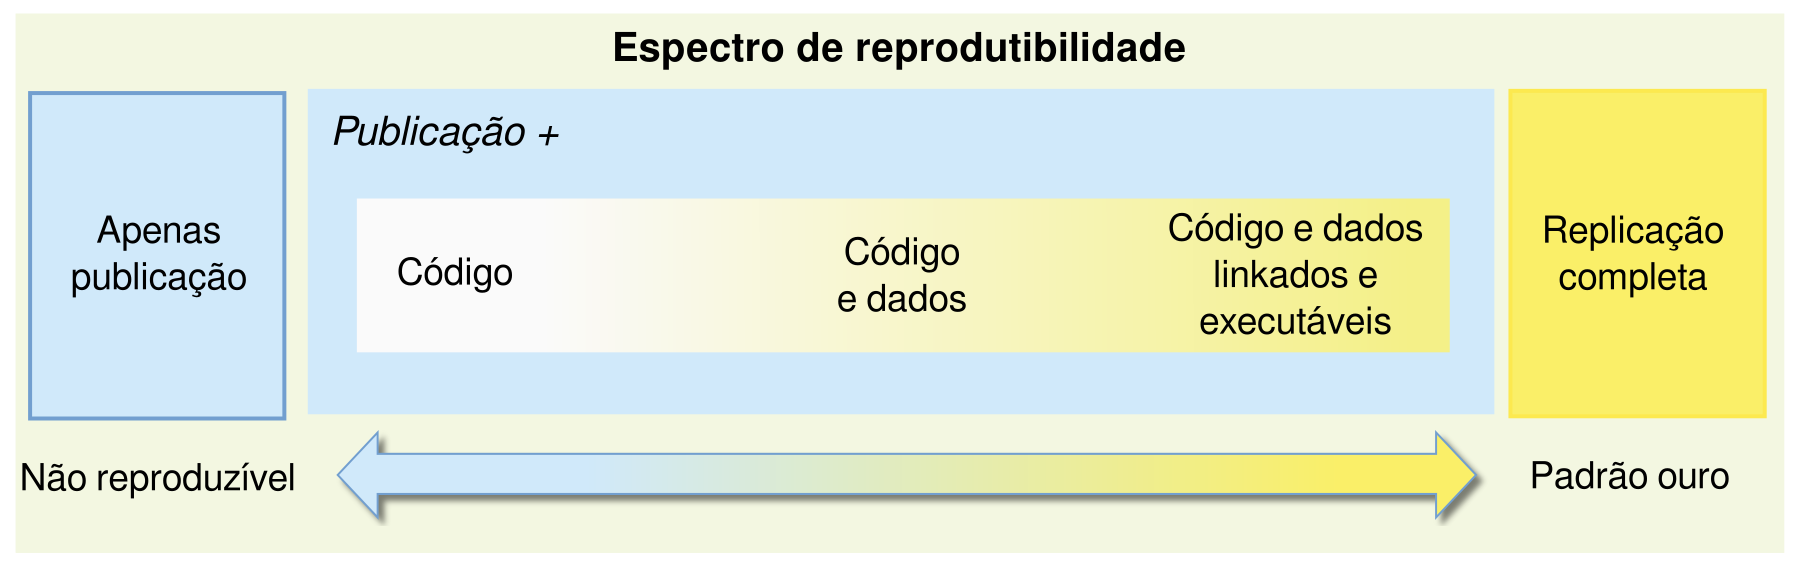
\includegraphics[scale=0.35]{imagens/reproducibility-spectrum-ptbr.png}
%  \caption{Espectro de reprodutibilidade \cite{Peng2011}}
%  \label{reproducibility-spectrum}
%\end{figure}

\subsection{Ciberinfraestrutura}

A visão da ciberinfraestrutura, expressada no "Relatório Atkins" e instanciada
para o ecossistema de software científico na NSF chamada de Infraestrutura de
Software para Inovação Sustentada (NSF SI2),
os softwares vem não apenas atuando no avanço da ciência, mas atuando com uma
eficiência crescente ao longo do tempo (Atkins 2003). A chave para isso é a
crença de que o software deve evoluir em direção a uma plataforma
compartilhada, com componentes que são reutilizados o mais amplamente possível,
já que os usuários finais e os produtores de componentes se agrupam em torno de
peças específicas de software.

%a literatura sobre plataformas de software fora da ciencia tem chamado isso de
%'coring' e 'tipping' (Gawer and Cusumano 2008),
%onde uma comunidade descobre sua funcionalidade compartilhada e se agrupa
%em pacotes que fornecem, levando ao uso eficiente de recursos através de
%economias de escala.

%coring também resulta em um aumento do uso sobreposto que facilita mais

%Isto também resulta em um aumento do uso sobreposto que facilita mais
%transparência na ciência, levando a uma maior qualidade e correctude (correctness), à medida
%que mais olhos e esforços são direcionados para os mesmos códigos que são
%sustentados e evoluem em longos períodos de utilidade científica.

%coring em direção às plataformas pode ser contrastado com o seu oposto, muitas
%vezes percebido por informantes: churn caótico disfuncional, com muitos
%projetos com poucos usuários, cada um tendo vidas curtas que terminam com o
%financiamento de concessão inicial, comunidades desconectadas e paralelas,
%incompatibilidades teimosamente imutáveis e periódicas e tentativas
%aparentemente não coordenadas de "reiniciar". Subjacente a isso é uma
%preocupação que as oportunidades são perdidas e que o progresso da ciência é
%abrandado (por exemplo, Stewart, Almes e Wheeler 2010).

%Assim, surge um conjunto de ações que podem ser tomadas pelos diferentes atores
%em direção à garantir sustentabilidade nos projetos de software, ações para
%praticantes de software, pesquisadores, associações profissionais, educadores,
%cientes e usuários.

%Inevitavelmente alguns softwares irão continuar sendo úteis após o primeiro
%release, alguns terão algums gerações de melhorias, outros serão usados na sua
%versão original sem atualização ou manutenção, e alguns outros irão ser
%lançados e nunca utilizados. Isto é perfeitamente natural, a comunidade ao
%redor do software irá decidir qual é o melhor caminho a se tomar num processo
%evolutivo \cite{weiner2009astronomical}.

%lugar, em algum momento. Uma utilidade óbvia para qualquer um destes softwares
%é para aqueles que desejam replicar as pesquisas em que foram criados, seja com
%o simples objetivo de validar as conclusões, seja com interesse de estender e
%colaborar com a pesquisa original.

\subsection{Pesquisas reproduzíveis}

Apesar das pesquisas reproduzíveis ({\it RR - Reproducible Research}) não
resolverem todos os problemas de validade experimental dos estudos em
engenharia de software, elas ao menos garantem que dados e métodos de análise
estejam disponíveis para inspeção e que os resultados possam ser derivados,
facilitando revisão logo que a publicação acontece. Além disso, é um recurso
valoroso para pesquisadores iniciantes, pesquisas reproduzíveis melhoram o
impacto do próprio estudo, por exemplo, artigos de computação que não
disponibilizam pubicamente dados e códigos possuem menos chances de serem
citados \cite{madeyski2017would}.

\subsection{Artigos executáveis}

Linked Open Science—Communicating, Sharing and Evaluating
Data, Methods and Results for Executable Papers.
Linked Open Science is an approach to solve challenges of an executable paper. It is a combination of four “silver
bullets”: 1) publication of scientific data, metadata, results, and provenance information using Linked Data principles,
2) open source and web-based environments for executing, validating and exploring research, 3) Cloud Computing
for efficient and distributed computing, and 4) Creative Commons for the legal infrastructure. We will use a realistic
scientific research setting related to research on deforestation of the Brazilian Amazon rainforest to provide scenarios
to illustrate the application of Linked Open Science \cite{kauppinen2011linked}.

\subsection{Software como cidadão de primeira classe}

JOSS, Papers executáveis, pesquisas reproduzíveis, etc, dar credibiidade ao
pesquisador cientista desenvolvedor de software ... papel do software na
reprodutibilidade, etc...

Apesar do reconhecimento de vários destes problemas nas mais diversas
áreas da ciência, ainda não sabe-se como o ecossistema de software
acadêmico de análise estática se posiciona neste cenário.

%%%%%%%%%%%%%%%%%

%Diversas maneiras de inventivar citação formal entre artefatos digitais,
%software por exemplo, tem surgido, dentre elas uma iniciativa interessante
%é o Journal of Open Source Software (JOSS) é um livre a open-access jornal para
%publicação de artigos descrevendo software acadêmico. Ele tem dois objetivos
%principais, melhorar a qualidade dos softwares submetidos e prover mecanismos
%para pesquisadores desenvolvedores de software acadêmico receber crédito pelos
%seus softwares. Enquanto pensado para trabalhar dentro do atual sistema de
%mérito da ciência, JOSS visa a escassez de recompensas para contribuições
%importantes para a ciência realizadas em forma de software. JOSS publica
%artigos que encapsulam sabedoria contida no software ele mesmo, e seu rigoroso
%revisão em pares mirado nos componentes do software: funcionalidade,
%documentação, testes, integração contínua, e a licença. Um artigo JOSS contém
%um resumo descrevendo o objetivo e funcionalidades do software, referencias, e
%um link para o software archive.  O artigo é um ponto de entrada para
%submissçao que engloba o conjunto completo de artefatos de software. Artigos
%aceitos no JOSS recebem um digital object identifier (DOI), te seus metadados
%depositados no Crossref, e o artigo pode começar a colecionar citações e ser
%indexados em serviços como Google Scholar e outros. No seu primeiro ano,
%iniciado em Maio de 2016, JOSS publicou 111 artigos, com mais de 40 artigos
%adicionais sob revisão \cite{smith2017journal}.

%FORCE11 Software Citation principles \cite{smith2016software}\footnote{\url{https://www.force11.org/software-citation-principles}}
%Enfatiza persistencia e claridade e diz que ``Software deve ser considerado
%um produto legítimo de pesquisas e devem ser possível de serem citados''.

%\item Reproducibility manifesto \cite{Barba2012}\footnote{\url{http://lorenabarba.com/gallery/reproducibility-pi-manifesto}}
%Inclui termos para fazer softwares reusáveis por outros. Foco em
%reprodutibilidade, deixando sustentabilidade de software fora de questão.

% Software Carpentry: lessons learned [version 2; referees: 3 approved]
%
% iniciativa voltada a melhorar as habilidades com computação entre os
% pesquisadores de diversas áreas, ajudando a melhorar os resultados,
% facilitar reprodutiblidade, acesso a dados, codigos, etc... reducao de custos
% melhoria de qualidade, etc... faz workshops, eventos, treinamentos, ao longo
% dos varios anos de existencia, ...
%
% Since its start in 1998, Software Carpentry has evolved from a week-long
% training course at the US national laboratories into a worldwide volunteer effort
% to improve researchers' computing skills. This paper explains what we have
% learned along the way, the challenges we now face, and our plans for the
% future.

% (6) A systematic literature review of software product line management tools \cite{pereira2015systematic}
%
% (???)
%
% (7) Software configuration management tools \cite{chan1997software}
%
% (???)

%A situação com software é amplamente análoga (mas não identica) ao de dados
%das publicações; de fato, todo dado é processado por softwares de alguma forma
%(Borgman et al., 2012).

%\item The GeoScience paper of the future initiative \cite{OntoSoft2016}\footnote{\url{http://www.scientificpaperofthefuture.org/gpf/what-is-a-gpf}}
%Possui um conjunto de requerimentos para softwares serem incluidos em
%papers.  Focando mais no paper em sí do que no software.

%\item UK RSE \cite{ukrse2013}\footnote{\url{http://rse.ac.uk/who}}
%Conscientização sobre a importância e o papel do {\it Research Software
%Engineer} através de comunicação e suporta institucional.

%Science rests on peer review and the wide-spread dissemination of
%knowledge. Software engineering research will advance further and
%faster if the sharing of data and tools were easier and more wide-
%spread. Pragmatic concerns hinder the realization of this ideal: the
%time and effort required and the risk of being scooped. We examine
%the costs and benefits of facilitating sharing in our field in an effort
%to help the community understand what problems exist and find
%a solution. We examine how other fields, such as medicine and
%physics, handle sharing, describe the value of sharing for replication
%and innovation, and address practical concerns such as standards
%and warehousing. To launch what we hope will become an ongoing
%discussion of solutions in our community, we present some ways
%forward that mitigate the risk of sharing — partial sharing, registry,
%escrow, and market \cite{barr2010shoulders}.

%Abstract—This paper is the result of reviewing all papers
%published in the proceedings of the former International
%Workshop on Mining Software Repositories (MSR) (2004-2006)
%and now Working Conference on MSR (2007-2009). We have
%analyzed the papers that contained any experimental analysis
%of software projects for their potentiality of being replicated.
%In this regard, three main issues have been addressed: i) the
%public availability of the data used as case study, ii) the public
%availability of the processed dataset used by researchers and iii)
%the public availability of the tools and scripts. A total number of
%171 papers have been analyzed from the six workshops/working
%conferences up to date. Results show that MSR authors use
%in general publicly available data sources, mainly from free
%software repositories, but that the amount of publicly available
%processed datasets is very low. Regarding tools and scripts, for
%a majority of papers we have not been able to find any tool,
%even for papers where the authors explicitly state that they have
%built one. Lessons learned from the experience of reviewing the
%whole MSR literature and some potential solutions to lower the
%barriers of replicability are finally presented and discussed
%\cite{robles2010replicating}.

%A survey of controlled experiments in software engineering
%Among
%the 20 replications, five can be considered as close replica-
%tions in the terminology of Lindsay and Ehrenberg [31], i.e.,
%one attempts to retain, as much as is possible, most of the
%known conditions of the original experiment.

%Replication of empirical studies in software engineering: Preliminary findings from a systematic mapping study
%The number of replications grew in the last few years, but the
%absolute number of replications is still very small, in particular
%considering the breadth of topics in software engineering. Incentive
%to perform external replications and better standards to report
%empirical studies and their replications are still needed.

%A ciência aberta e comunidades de pesquisa em software tem sido bastante ativas
%em criar manifestos visando chamadas para ação. Estes manifestos chamam para melhorar
%os softwares e os metadados de bibliografia para citação persistente destes softwares.
%Outros tópicos endereçados nestes manifestos incluem ênfase no acesso ao código fonte.

%Muitos estudos em engenharia de software sofrem de dificuldades de repetição
%\cite{Tang2016}, artigos citando desenvolvimento de scripts ou protótipos
%apresentam chance próximo a nulo de terem tais artefatos disponíveis, a
%replicabilidade das pesquisas tendem a cair com a idade da publicação, páginas
%ou repositórios se tornam indisponíveis com o passar do tempo
%\cite{robles2010replicating}, não se sabe como as taxas de softwares
%disponíveis, executáveis, e escondidos ({\it hidden software}) mudam ao longo
%do tempo \cite{allen2017engineering}, softwares acadêmicos são, muitas vezes, mal
%documentados, não intuitivos e difíceis de instalar, uma fração substancial são
%abandonware, ou seja, não são mais mantidos ou desenvolvidos ativamente, mesmo
%tendo um valor potencial para a comunidade científica \cite{list2017ten}.

%Isto contradiz as boas práticas de qualquer projeto experimental ({\it
%laboratory
%notebooks}\footnote{\url{https://en.wikipedia.org/wiki/Lab_notebook}}, dados
%organizados, passos documentados, projeto estruturado para reprodutibilidade) e
%torna praticamente impossível utilizar o método mais comum e cientificamente
%produtivo de produzir conhecimento novo a partir de pesquisas anteriores, a
%replicação, ou seja, seguir os mesmos passos do autor original com
%objetivo de validar, melhorar ou estender seus dados e sua metodologia
%\cite{king1995replication, Stodden2010}.

%estas práticas permitem replicar descobertas anteriores seguindo
%o caminho do autor original,
%isto, segundo
%
% Replicability is not Reproducibility: Nor is it Good Science
%
% I want to challenge this view by separating
% the notion of reproducibility, a generally de-
% sirable property, from replicability, its poor
% cousin. I claim there are important differ-
% ences between the two. Reproducibility re-
% quires changes; replicability avoids them. Al-
% though reproducibility is desirable, I contend
% that the impoverished version, replicability,
% is one not worth having.
% ...
% In this paper, I have claimed that what many in the
% field are advocating is the replicability of published
% experiments. They argue that this meets the repro-
% ducibility requirement inherent to science. My claim
% is that replicability is a poor substitute for scientific
% reproducibility. There may be other good reasons for
% the collecting of software and scripts that are the ba-
% sis of the experimental results published in papers but
% scientific reproducibility is not one.
%
%The lack of replicability and reproducibility of scientific studies based on
%computational methods has lead to serious mistakes in published scientific
%findings, some of which have been discovered and publicized recently. Many
%strategies are currently pursued to improve the situation. This article reports the
%first conclusions from the ActivePapers project, whose goal is the development
%and application of a computational platform that allows the publication of
%computational research in a form that enables installation-free deployment,
%encourages reuse, and permits the full integration of datasets and software into
%the scientific record. The main finding is that these goals can be achieved with
%existing technology, but that there is no straightforward way to adapt legacy
%software to such a framework \cite{hinsen2014activepapers}
%
%% Ainda existem poucos estudos replicados \cite{kitchenham2015evidence}.

% Em resumo os dois manifestos, Dagstuhl e Karlskrona, exprimem o conceito de
% sustentabilidade necessários para este estudo, mas é importante citar que
% algumas iniciativas e outros manifestos também estão preocupados com questões
% similares, dentre os quais podemos destacar:

%A ciência aberta e comunidades de pesquisa em software tem sido bastante ativas
%em criar manifestos visando chamadas para ação. Estes manifestos chamam para melhorar
%os softwares e os metadados de bibliografia para citação persistente destes softwares.
%Outros tópicos endereçados nestes manifestos incluem ênfase no acesso ao código fonte.

% Software Sustainability: The Modern Tower of Babel

%Somado a isto temos ainda o fato de que pesquisadores raramente publicam seus
%códigos, piorando ainda mais toda a situação, isto tem motivado a organização
%de conferências específicas para discutir os problemas dos softwares
%acadêmicos, como o RSE (Conference of Research Software Engineers)\footnote{
%\url{http://rse.ac.uk/conf2017}}, WSSSPE (Workshop on Sustainable Software for
%Science: Practice and Experiences)\footnote{
%\url{http://wssspe.researchcomputing.org.uk}} e o RESER (Workshop on
%Replication in Empirical Software Engineering Research)\footnote{
%\url{http://sequoia.cs.byu.edu/reser}}, e tem agregado discussões das
%comunidades de ciência aberta, reprodutibilidade e sustentabilidade de
%software.

%A ciência caminha sob a teoria e experimentação \cite{vardi2010science}. Não existe ciência fechada.

%Há uma explosão de dados abertos disponíveis on-line que é acessado e analisado
%através da criação de um novo software - gerando mais dados para analisar. Os
%softwares, ou seja, qualquer software que adquira, limpe, armazene, anote,
%transforme, filtre, gere (etc.) dados de pesquisa.

%\section{Seção sem nome ainda}

%Estes são alguns problemas relacionados aos softwares acadêmicos, muitos são
%resultado de baixos orçamentos, limitação de tempo e alta rotatividade entre os
%grupos de pesquisa, outros são, possivelmente, ocasionados por questões
%culturais \cite{niemeyer2017open}, como, por exemplo, a tímida adoção de
%práticas da ciência aberta entre pesquisadores. Compreender os reais motivos
%por trás destes problemas seria, naturalmente, o passo essencial para solucioná-los,
%apesar disso, antes mesmo de resolver tais questões é
%fundamental compreender os impactos que eles causam na comunidade de pesquisa.

%Isto se torna ainda mais difícil visto que frequentemente os pesquisadores
%deixam de publicar o código dos seus softwares acadêmicos argumentando que o
%código é ``ruim'' e isto irá gerar julgamentos negativos ao pesquisador
%\cite{allen2017engineering}.

%Os compromissos expressados neste manifesto são agrupados em três conceitos gerais:
%(i) garantir que softwares científicos sejam {\it citados} apropriadamente;
%(ii) promover a {\it carreira} do engenheiro de software desenvolvedor de software científico; e
%(iii) medir a qualidade e sustentabilidade do software científico durante e após o seu {\it desenvolvimento}.

%um caminho apontado como solução é acreditar que software deve evoluir para plataformas compartilhadas,
%com componentes reusáveis tanto quanto possível, tanto para usuário final, quanto
%para produtores de componentes (papel) agregando peças particulares de software,
%crença de que o software deve evoluir em direção a uma plataforma
%compartilhada, com componentes que são reutilizados o mais amplamente possível,
%já que os usuários finais e os produtores de componentes se agrupam em torno de
%peças específicas de software.

%Essa definição de sustentabilidade de software é encontrada em mais detalhes no
%{\it Karlskrona Manifesto} \cite{becker2014karlskrona}, um documento que alerta
%sobre os impactos que os sistemas e a tecnologia da informação causam no futuro
%do planeta, convida praticantes e pesquisadores de software a refletir sobre
%o tema sustentabilidade na área da ciência da computação.

%Reproducibility verification is essential to the practice of the scientific method.
%Researchers report their findings, which are strengthened as other independent groups
%in the scientific community share similar outcomes. In the many scientific fields
%where software has become a fundamental tool for capturing and analyzing data, this
%requirement of reproducibility implies that reliable and comprehensive software platforms
%and tools should be made available to the scientific community. The tools will empower
%them and the public to verify, through practice, the reproducibility of observations that
%are reported in the scientific literature. Medical image analysis is one of the fields in
%which the use of computational resources, both software and hardware, are an essential
%platform for performing experimental work. In this arena, the introduction of the Insight
%Toolkit (ITK) in 1999 has transformed the field and facilitates its progress by accelerating
%the rate at which algorithmic implementations are developed, tested, disseminated and
%improved. By building on the efficiency and quality of open source methodologies, ITK has
%provided the medical image community with an effective platform on which to build a daily
%workflow that incorporates the true scientific practices of reproducibility verification. This
%article describes the multiple tools, methodologies, and practices that the ITK community
%has adopted, refined, and followed during the past decade, in order to become one of the
%research communities with the most modern reproducibility verification infrastructure. For
%example, 207 contributors have created over 2400 unit tests that provide over 84% code
%line test coverage. The Insight Journal, an open publication journal associated with the
%toolkit, has seen over 360,000 publication downloads. The median normalized closeness
%centrality, a measure of knowledge flow, resulting from the distributed peer code review
%system was high, 0.46 \cite{McCormick2014}.

%Among empirical software engineering studies, those based on data re-
%trieved from development repositories (such as those of source code management,
%issue tracking or communication systems) are specially suitable for reproduction.
%However their reproducibility status can vary a lot, from easy to almost impossible
%to reproduce. This paper explores which elements can be considered to characterize
%the reproducibility of a study in this area, and how they can be analyzed to better
%understand the type of reproduction studies they enable or obstruct. One of the
%main results of this exploration is the need of a systematic approach to asses the
%reproducibility of a study, due to the complexity of the processes usually involved,
%and the many details to be taken into account. To address this need, a methodology
%for assessing the reproducibility of studies is also presented and discussed, as a tool to
%help to raise awareness about research reproducibility in this field. The application
%of the methodology in practice has shown how, even for papers aimed to be
%reproducible, a systematic analysis raises important aspects that render reproduction
%difficult or impossible. We also show how, by identifying elements and attributes
%related to reproducibility, it can be better understood which kind of reproduction
%can be done for a specific study, given the description of datasets, methodologies and
%parameters it uses \cite{gonzalez2012reproducibility}.

%At various machine learning conferences, at
%various times, there have been discussions
%arising from the inability to replicate the
%experimental results published in a paper.
%There seems to be a wide spread view that we
%need to do something to address this prob-
%lem, as it is essential to the advancement
%of our field. The most compelling argument
%would seem to be that reproducibility of ex-
%perimental results is the hallmark of science.
%Therefore, given that most of us regard ma-
%chine learning as a scientific discipline, being
%able to replicate experiments is paramount.
%I want to challenge this view by separating
%the notion of reproducibility, a generally de-
%sirable property, from replicability, its poor
%cousin. I claim there are important differ-
%ences between the two. Reproducibility re-
%quires changes; replicability avoids them. Al-
%though reproducibility is desirable, I contend
%that the impoverished version, replicability,
%is one not worth having \cite{drummond2009replicability}.

%Over the past fifteen years the scholarly communications agenda
%has progressed gradually. Currently we are experiencing a strong
%tendency among all research stakeholders to engage with the
%practice of OS. Lately, research funders require the sharing not
%only of the research results they have funded, but also of the
%procedures and data that are being generated during the research
%conduct. Researchers, on the other side, are keen on observing
%their research results being used for the improvement of the
%society and are forced by their funders to demonstrate the impact
%of their research. At the same time, higher academic institutions
%aim to join the OS agenda as well, since they see the opportunity
%of great economic benefits and savings. While OS is the possible
%answer to all these factors, the stakeholders’ inability to
%understand the requirements for the application of OS can be a
%suspensory factor for the OS implementation and evolution.
%The aim of the FOSTER project is to advance the stakeholders'
%knowledge on the usefulness of OS and explain the technicalities,
%strategies and best practices using which OS can be applied. As an
%attempt to educate the largest number of researchers possible,
%FOSTER has created an e-leanring portal, which contains quality
%assured information relating to the topic and it is open to everyone
%in the world. The platform contains two types of information:
%learning material and online courses. The classification of these
%two types is supported by an OS taxonomy, where related terms
%are applied both in the portal's material and also in the courses.
%With the use of the taxonomy, users are in the position to
%understand the OS domain and the concepts around it.
%The main goal of the FOSTER project, which is mainly achieved
%through the portal functionalities, is not only to educate the
%research stakeholders on OS, but also to build a community of
%researchers, librarians, software developers, funders and research
%administrators who are interested in OS in order to advance the
%way research is being conducted and shared. In addition, FOSTER
%attempts to provide tools to this community, such as re-usable
%content for training and a platform for blended learning and e-
%learning courses that the community could run. This OS
%advancement is essential for the research promotion and,
%consequently, for the benefit of the society as a whole
%\cite{Nancy2015}.
%
%Open Science may be practised both
%for philosophical and pragmatic reasons. As the
%resources produced by open projects are
%potentially accessible to public audiences, Open
%Science offers both a novel medium for public
%access and involvement in the process of science
%and an innovative method for real-time science
%communication. Does such direct access clear
%the stream of communication or muddy the
%waters with unfocussed, unclear and unvetted
%comment? This paper suggests that adopting an
%Open Science approach allows the capture of an
%authentic and clear record of research.
%However, researchers acknowledge this involves
%opening their work up to a different type of
%scrutiny \cite{Grand2010}.
%
%Open Science is an emerging approach to the conduct of science, technology and engineering
%projects, in which information about the whole of an ongoing investigation is made available
%on and through the Internet. Adopting an Open Science approach means the audience for the
%research can extend beyond the researchers involved to other researchers and to members of
%the public. Thus, Open Science has implications for engineering research, practice,
%publishing and public engagement with engineering. This paper reviews the history and
%evolution of the Open Science movement, includes some reflections on the related areas of
%Open Access, peer-review and public engagement with science and engineering and discusses
%data gathered from interviews. The analysis suggests that interviewees have concerns about
%issues such as precedence and protection of original work and the time needed to integrate
%open science practices into daily work. Successfully working in such collaborations is likely
%to require not only common practical tools but also the development of shared language and
%understanding between researchers and members of the public. Interviewees recognise the
%value of Open Science in collaborative research and its innovative facility to sustain direct
%public access to research outputs. It also has the potential to allow members of the public to
%make real practical contributions to research \cite{Grand2010Open}.
%
%This white paper was written as a contribution to the “Imagining
%Tomorrow’s University: Rethinking scholarship, education, and institu-
%tions for an open, networked era” workshop, a joint NIH/NSF-funded
%event held 8–9 March 2017 in Rosemont, IL. In this paper, I present an
%overview of what I consider open science, its importance, and how it
%plays a role in my research agenda. I also discuss challenges faced in
%pursuing research openness, and recommend changes to university
%leaders to address these barriers \cite{niemeyer2017open}.
%
%Open to All?  Case studies of openness in research
%Since the early 1990s, the open access movement has promoted the concept of openness in relation
%to scientific research. Focusing initially upon the records of science in the form of the text of articles
%in scholarly journals, interest has broadened in the last decade to include a much wider range of
%materials produced by researchers. At the same time, concepts of openness and access have also
%developed to include various kinds of use, by machines as well as humans.
%Academic bodies, including funders and groups of researchers, have set out statements in support
%of various levels of openness in research. Such statements often focus upon two key dimensions:
%what is made open, and how; and to whom is it made open, and under what conditions? This study
%set out to consider the practice of six research groups from a range of disciplines in order to better
%understand how principles of openness are translated into practice \cite{Nesta2010}.

%chape para isto é acreditar que software deve evoluir para plataformas compartilhadas,
%com componentes reusáveis tanto quanto possível, tanto para usuário final, quanto
%para produtores de componentes (papel) agregando peças particulares de software

% fez exatamente o que pensei, vou ler para usar a metodologia "adaptada"
%In addition to these motivation studies, scientists have recently embarked on the issue of
%software use and impact. A study in 2013 has found that scientists tend to choose software
%that is widely used by others in their community and prefer software that is free for
%academic use (Huang et al. 2013). Studies on the scientific software ecosystem have
%suggested that the use of scientific software is influenced by its visibility, availability,
%sustainability, reproducibility, and citation (Howison and Herbsleb 2014; Howison et al.
%2015; Huang et al. 2013). Studies also have suggested that software developers are
%interested to know the use and impact of their software because ‘‘software use matters to
%them for funding purposes’’ (Howison et al. 2015; Trainer et al. 2015, p. 428).
%Recent studies on data impact have led to the discussions on software citation and
%evaluation, as a parallel can be drawn between software and data in scientific literature
%(Piwowar et al. 2011; Howison and Bullard 2016). It is suggested that the numbers of
%mentions and citations in literature can be used to measure the impact of software (Huang
%et al. 2013; Pan et al. 2015). Yet, it is argued that ‘‘the practices of citation to software vary
%considerably from field to field and appear to miss significant software’’ (Howison et al.
%2015, p. 478). One study examining the use of software in scientific articles in biology has
%found that more than half of the software mentions did not include references (Howison
%and Bullard 2016). Thus, it validates the need to use alternative metrics in addition to
%citations when assessing software impact, such as the numbers of downloads, registered
%users, subscribers, user reviews, and artifacts inserted in literature (Howison et al. 2015).

% Ten Simple Rules for Reproducible Computational Research
% \cite{sandve2013ten}
%
% NumFOCUS is a 501(c)(3) nonprofit that supports and promotes world-class,
% innovative, open source scientific computing.
% https://www.numfocus.org/
